\documentclass[12pt,letterpaper,noanswers]{exam}
\usepackage[usenames,dvipsnames,svgnames,table]{xcolor}
\usepackage[margin=0.9in]{geometry}
\renewcommand{\familydefault}{\sfdefault}
\usepackage{multicol}
\usepackage{wrapfig}
\pagestyle{head}
\definecolor{c03}{HTML}{FFDDDD}
\header{AM 22b Class 20}{}{Mar 17: Flow in a vector field p.\thepage}
\runningheadrule
\headrule
\usepackage{graphicx} % more modern
\usepackage{amsmath} 
\usepackage{amssymb} 
\usepackage{hyperref}
\usepackage{tcolorbox}
\usepackage[utf8]{inputenc}
\pagenumbering{arabic}

\usepackage[numbered,autolinebreaks,useliterate]{mcode}

\newcommand{\mb}[1]{\underline{#1}}

\begin{document}
 \pdfpageheight 11in 
  \pdfpagewidth 8.5in




% I need to review the torus trajectories...

\begin{itemize}
% \item There is a pre-class assignment (20 minutes of videos + a few WeBWorK exercises) due at 10am this Monday.  It is available on Canvas.
\itemsep0em
    \item Quiz 03 will be posted on Friday.
    \item The skill check for C19, 20, 21 will be on Monday.
    \item There is a discussion board assignment due tomorrow.
    \item My OH are happening as scheduled today and Eva has extra OH tomorrow 7-8pm.
\end{itemize}

\hrule
\vspace{0.2cm}

\noindent\textbf{Big picture}

Today is focused on flow lines: parameterized curves that match up with a vector valued function in a special way.  Specifically these are parameterized curves where the velocity vector along the curve is equal to the value of the vector valued function at points along the curve.

\vspace{0.2cm}
\hrule
\vspace{0.2cm}



\noindent\textbf{Skill Check C20 Practice}
\begin{questions}
\question For $\mb v = x\mb i + y\mb j$,
\begin{parts}
\item find the system of differential equations associated with the vector field.
\item Does the flow $x(t) = ae^t, y(t) = be^{-t}$ satisfy the system?  \emph{Show your calculation steps}

\begin{oneparcheckboxes}
\choice yes
\choice no
\end{oneparcheckboxes}
\end{parts}
\end{questions}


\vspace{0.2cm}
\hrule
\vspace{0.2cm}

\noindent\textbf{Skill Check C20 Practice Solution}
\begin{questions}
\question 
\begin{parts}
\item $\frac{dx}{dt} = x, \frac{dy}{dt} = y$.
\item $x(t) = ae^t$ so $\frac{dx}{dt} = ae^t$.  Does this satisfy $\frac{dx}{dt} = x$?  Yes: $ae^t=ae^t$.  $y(t) = be^{-t}$ so $\frac{dy}{dt} = -be^{-t}$.  Does this satisfy $\frac{dy}{dt}$?  No: $be^{-t} \neq -be^{-t}$.
\end{parts}
\end{questions}

\vspace{0.2cm}
\hrule
\vspace{0.2cm}

\noindent\textbf{Teams}

You will work with this team on the in-class problems today.
\begin{multicols}{2}

1.  students here

\end{multicols}

%\vspace{0.2cm}
\hrule
\vspace{0.2cm}


\noindent\textbf{Velocity vector fields: flow lines} \S 17.4
\begin{tcolorbox}
\begin{itemize}
\itemsep0em
    \item Let $\mb v(x,y) = \langle f(x,y), g(x,y)\rangle$ be a vector field.  Choose a point $\mb{x_0} = (x_0,y_0)$ in the domain of $\mb F$.  There is a \textbf{flow line}, $\phi_t(\mb{x_0})$, passing through $\mb{x_0}$ where the velocity vector at each point on the path is equal to $\mb v$ at that point.
    % \item Consider a flow line $\phi_t(\mb{x_0})$.  Let $\langle x(t),y(t)\rangle = \phi_t(\mb{x_0})$.  On the flow line, we have $\frac{d\langle x(t), y(t)\rangle}{dt} = \mb v(x(t),y(t))$.  More explicitly, $\displaystyle \left(\begin{array}{c} dx/dt \\ dy/dt \end{array}\right) = \left(\begin{array}{c}f(x(t),y(t)) \\ g(x(t),y(t))\end{array}\right)$.
    \item The \textbf{flow}, $\phi(t,\mb{x})$, of a vector field is the family of all of its flow lines.
\end{itemize}
\end{tcolorbox}

\eject
\noindent\textbf{Example}

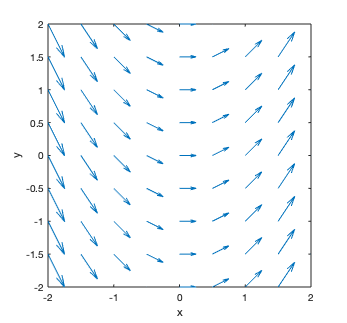
\includegraphics[width=0.45\linewidth]{img/C19vectorfield.png}
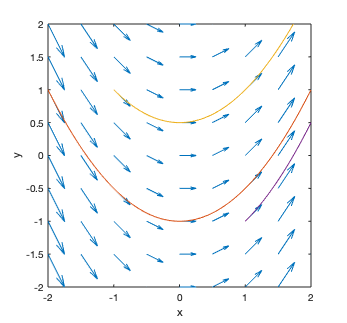
\includegraphics[width=0.45\linewidth]{img/C19vectorfieldflow.png}

On the left, I've plotted the vector field $\mb v = \langle 1, x\rangle$.  On the right, I've added three flow lines: $\phi_t(\mb{x_0})$ for $\mb{x_0} = (-2, 1)$ (red), $\mb{x_0} = (-1,1)$ (yellow), $\mb{x_0} = (1,-1)$ (purple).

\begin{lstlisting}
% Put x and y in the rows of a matrix.
% (the flow line function will use rows)
% Using a ";" as in [1; 2] creates a 2x1 matrix
% Using a "," as in [1, 2] creates a 1x2 matrix

fc = @(t,xy) [1+0*xy(1,:); xy(1,:)]; 
% t needs to be an input for this function to work
% with the function we will use to generate flow lines.
% the input xy has two rows (the x and y coordinates)
% xy(1,:) is the x-coordinate info.

% make a grid of (x,y) points for plotting the vector field.
xval = -2:0.5:2;
[xv,yv] = meshgrid(xval,xval);
% create a matrix with two rows that hold all the xy pairs:
xypairs = [xv(:)'; yv(:)'];
% make the vectors of the vector field:
vectors = fc(0, xypairs);
% plot the vector field:
quiver(xypairs(1,:),xypairs(2,:),vectors(1,:),vectors(2,:))
axis equal
axis([-2 2 -2 2])
xlabel('x'); ylabel('y');
\end{lstlisting}

\vspace{0.2cm}
\hrule
\vspace{0.2cm}

\noindent\textbf{Velocity vector fields: checking for a flow line} \S 17.4
\begin{tcolorbox}
 Given a curve, $\langle x(t), y(t)\rangle$, and a vector field $\mb v(x,y) = \langle f(x,y), g(x,y)\rangle$, the curve is a flow line of the vector field when $dx/dt = f(x,y)$ and $dy/dt = g(x,y)$ at every point along the curve.
\end{tcolorbox}

\eject

\noindent\textbf{Example: match flow lines to a vector field}

Consider the vector field $\mb v = \left(\begin{array}{r}-y \\ x\end{array}\right)$.  We have $f(x,y) = -y$ and $g(x,y) = x$.

Which of the following equations parameterize a family of flow lines for this vector field?
\begin{enumerate}
\itemsep2em
    \item $\left(\begin{array}{r}x(t) \\ y(t)\end{array}\right)=\left(\begin{array}{r} a\sin t \\ a\cos t\end{array}\right)$
     \item $\left(\begin{array}{r}x(t) \\ y(t)\end{array}\right)=\left(\begin{array}{r} a\cos t \\ a\sin t\end{array}\right)$
     \item $\left(\begin{array}{r}x(t) \\ y(t)\end{array}\right)=\left(\begin{array}{r} -a\sin t \\ a\cos t\end{array}\right)$
\end{enumerate}
\vspace{0.5in}

\noindent\textbf{Example: match a vector field to flow lines}

Consider the family of parameterized curves $\left(\begin{array}{r}x(t) \\ y(t)\end{array}\right)=\left(\begin{array}{r} ae^t \\ be^{-t}\end{array}\right)$

For which of the following vector fields does this set of curves form the flow lines?

\begin{enumerate}
\itemsep2em
    \item $\mb v = \left(\begin{array}{r} x \\ y\end{array}\right)$
     \item $\mb v = \left(\begin{array}{r} x \\ -y\end{array}\right)$
     \item $\mb v = \left(\begin{array}{r} -x \\ y\end{array}\right)$
\end{enumerate}
\vspace{0.5in}

\vspace{0.2cm}
\hrule
\vspace{0.2cm}

\noindent\textbf{Velocity vector fields: finding a flow line} \S 17.4
\begin{tcolorbox}
\begin{itemize}
\itemsep0em
    \item Given a curve, $\langle x(t), y(t)\rangle$, and a vector field $\mb v(x,y) = \langle f(x,y), g(x,y)\rangle$, the curve is a flow line of the vector field when $dx/dt = f(x,y)$ and $dy/dt = g(x,y)$ at every point along the curve.
    \item The equations $dx/dt = f(x,y)$ and $dy/dt = g(x,y)$ form a \textbf{system of differential equations}.  Differential equations are equations in which the derivative of a function appears.  A solution to this system is a vector valued function $\langle x(t), y(t)\rangle$ that satisfies the equation.
\end{itemize}
 
\end{tcolorbox}

\noindent\textbf{Example (system of differential equations)}

Write down the system of differential equations associated with finding the flow for the vector field $\mb v = \langle y,x\rangle$.
\vspace{1in}

We will study differential equations later in the semester and will wait to find (or approximate) solutions to these systems until mid-April.


\vspace{0.2cm}
\hrule
\vspace{0.2cm}

\noindent\textbf{Velocity vector fields: showing flow lines lie on level curves} \S 17.4
\begin{tcolorbox}
\begin{itemize}
\itemsep0em
    \item Given a vector field, $\mb v(x,y) = \langle f(x,y), g(x,y)\rangle$, there may exist a function $h(x,y)$ such that the flow lines of $\mb v$ lie on level curves of $h(x,y)$.
    \item Given a function $h(x,y)$, level curves are of the form $h(x,y) = c$.  When a flow line lies on a level curve, $h(x(t),y(t)) = c$ for all values of $(x(t),y(t))$ along the flow line.
    
    Following the path $(x(t), y(t))$, we would have $\frac{dh}{dt} = 0$.
    
    %\displaystyle\frac{dh}{dt} = h_x x_t + h_y y_t$.  For flow lines of the vector field, $x_t = f(x,y)$ and $y_t = g(x,y)$, so in that special case we have $h_t = h_x f(x,y) + h_y g(x,y)$.  When we can show that $h_x f + h_y g = 0$
\end{itemize}
 
\end{tcolorbox}
% \begin{multicols}{2}

\noindent\textbf{Example}

Let $\mb v = \mb i + x \mb j$ and $h(x,y) = 2y-x^2$.
\begin{enumerate}
\itemsep4em
    \item Find the system of differential equations associated with the vector field.
    \item Use the chain rule to find $\dot h$ in terms of $x, y, \dot x, \dot y$.
    \item Along flow lines, $\dot x$ and $\dot y$ satisfy the system of differential equations.  Substitute that information to expression $\dot h$ in terms of $x$ and $y$.
    \item Simplify: are you able to show that $\dot h = 0$ along flow lines?
\end{enumerate}
\vspace{1cm}

\noindent\textbf{Example}

Show that every flow line of the vector field $mb v = ay\mb i + bx\mb j$ lies on a level curve of the function $h(x,y) = bx^2-ay^2$.
\vfill

% \end{multicols}


% \begin{lstlisting}
% %% Add a flow line.
% hold on
% timespan = [0,4];
% flowline = ode45(fc,timespan,[-2; 1]);

% tplot = linspace(min(timespan),max(timespan),100);
% output = deval(flowline,tplot);
% plot(output(1,:),output(2,:))
% axis equal
% axis([-2 2 -2 2])
% hold off
% \end{lstlisting}

\eject


\vspace{0.2cm}
\hrule
\vspace{0.2cm}

\noindent\textbf{Line integrals: length of a curve}.  \S 18.1  
\begin{tcolorbox}
\begin{itemize}
\itemsep0em
    \item Let $\mb r(t), a\leq t\leq b$ be a parameterization of an oriented curve $C$.  $\Vert \mb r(t)\Vert$ is the speed of motion along the curve.  $\Delta s = \Vert\mb r(t)\Vert \Delta t$ is the \textbf{approximate distance} moved along the curve in a time interval of $\Delta t$.
    \item An \textbf{oriented curve} is a curve where the direction of travel has been specified.
    \item A curve is \textbf{simple} if it does not cross itself.  Given a simple curve, there are two possible orientations.
    \item The \textbf{length of a curve} $C$ is given by $\int_C ds$ where $ds$ is the infinitesimal version of $\Delta s$.  Let $\mb r(t), a\leq t\leq b$ be a parameterization of $C$.  $\displaystyle\int_C ds= \int_a^b \left\Vert \mb r'(t)\right\Vert dt$.
\end{itemize}
\end{tcolorbox}

\noindent\textbf{Example: length of a curve}

Let the curve $C$ by the helix parameterized by $x(t) = \cos t$, $y(t) = \sin t$, $z(t) = t$, $0\leq t\leq 6\pi$.  Set up at integral to find the length of $C$.

To do this:
\begin{enumerate}
\itemsep2em
    \item Find $\mb v(t)$ for the parameterization.
    \item Find $\Vert \mb v(t)\Vert$, the speed of motion along the curve.
    \item Set up the integral of speed with respect to time.
    \item If feasible, integrate to compute the length of $C$.
\end{enumerate}
\vspace{1cm}

\vspace{0.2cm}
\hrule
\vspace{0.2cm}

\noindent\textbf{Line integrals: scalar function}.  \S 18.1  

\begin{tcolorbox}
\begin{itemize}
\itemsep0em
    \item A \textbf{line integral} is an integral where we integrate the value of a function along an oriented curve.
    \item A \textbf{line integral for a scalar field}, $f:\mathbb{R}^3 \rightarrow \mathbb{R}$, is given by \[\int_C f\ ds = \int_a^b f(\mb r(t)) \Vert \mb r'(t)\Vert dt\] with $\mb r(t), a\leq t\leq b$ a parameterization of $C$.
    \item A \textbf{scalar field} is a function with a single output.
\end{itemize}
\end{tcolorbox}


\href{https://upload.wikimedia.org/wikipedia/commons/4/42/Line_integral_of_scalar_field.gif}{\emph{click for illustrating gif}}


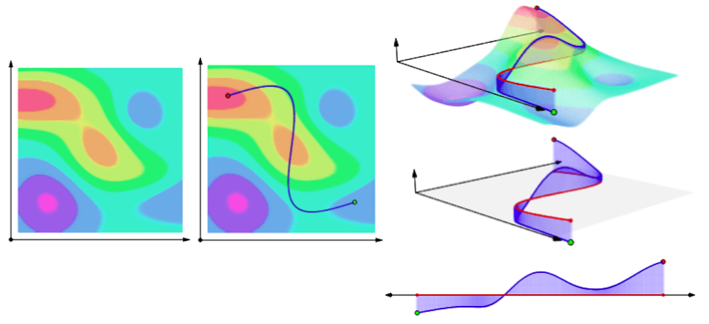
\includegraphics[width=\linewidth]{img/C25p1-18.png}
\url{https://upload.wikimedia.org/wikipedia/commons/4/42/Line_integral_of_scalar_field.gif}




\noindent\textbf{Example (mass).} 
Let $C$ be the shape of a wire parameterized by $x(t) = t, y(t) = t^2, 0\leq t\leq 1$.  Assume the wire has density $f(x,y) = k x^2$.  Rewrite the integral $\displaystyle\text{Mass} = \int_C f \ ds$ as an integral with respect to time.

\vfill


\vspace{0.2cm}
\hrule
\vspace{0.2cm}

\noindent\textbf{Line integral: vector field} \S 18.1
\begin{tcolorbox}
\begin{itemize}
\itemsep0em
    \item A \textbf{line integral for a vector field}, $\mb F:\mathbb{R}^3 \rightarrow \mathbb{R}^3$, along an oriented curve, $C$, is given by \[\int_C \mb F(\mb r)\cdot \mb T\ ds = \int_a^b \mb F(\mb r(t))\cdot \frac{d\mb r}{dt}\ dt\] where $\mb T$ is a unit vector in the direction tangent to $C$, and $\mb r(t)$ with $a\leq t\leq b$ is a parameterization of $C$. \href{https://upload.wikimedia.org/wikipedia/commons/b/b0/Line_integral_of_vector_field.gif}{\emph{click for illustrating gif}}
    \item Another notation for this is \[\int_C \mb F(\mb r)\cdot d\mb r = \int_a^b \mb F(\mb r(t)) \cdot \frac{d\mb r}{dt}dt\] with $\mb r(t), a\leq t\leq b$ a parameterization of $C$.
\end{itemize}



\tcblower

\begin{itemize}
\itemsep0em
    \item A line integral in a force vector field is used to compute the \textbf{work} done by a force to move an object (with mass or electric charge) along a path.

\item A \textbf{circulation} integral (a line integral where the curve $C$ is closed, denoted $\oint_C \mb F\cdot d\mb r$) is used to compute the circulation of a velocity vector field along a closed curve.  The circulation tells us about the net alignment of the vector field with the closed curve.

In the Kutta-Joukowski model of lift, circulation is an important component of modeling the lift force on an airplane wing.
\end{itemize}
\end{tcolorbox}

\noindent\textbf{Setting up a line integral}. 
Show that
\[\int_C \mb F(\mb r)\cdot \mb T\ ds = \int_a^b \mb F(\mb r(t))\cdot \frac{d\mb r}{dt}\ dt\] when the oriented curve $C$ is parameterized by $\mb r(t), a\leq t\leq b$. 
Recall that $\displaystyle\mb v = \frac{d\mb r}{dt}$, that $\displaystyle\mb T = \frac{\mb v}{\Vert\mb v\Vert},$ and that $\displaystyle ds = \Vert \mb v\Vert dt$.
\vspace{1in}


\noindent\textbf{Vector field vs scalar field}

Compare $\int_C f\ ds$ and $\int_C \mb F(\mb r)\cdot \mb T\ ds$.  $\mb F(\mb r)\cdot \mb T$ is a scalar.  What does it represent?

\hspace{-0.3in}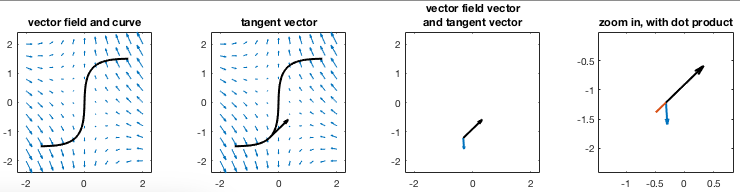
\includegraphics[width=0.8\linewidth]{img/C25p3-18.png}

\vspace{1in}


\noindent\textbf{Line integrals: identifying the sign} \S 18.1
\begin{tcolorbox}
\begin{itemize}
\itemsep0em
    \item Let $f(\mb r) = \mb F(\mb r)\cdot \mb T$.  If $f(\mb r)>0$ on $C$ then $\int_C f\ ds>0$.  If $f(\mb r)<0$ on $C$ then $\int_C f\ ds < 0$.  If $f(\mb r) = 0$ on $C$ then $\int_C f\ ds = 0$.  In these cases, the sign of the line integral can be identified without further reasoning.
    \item Sometimes $\mb F(\mb r)\cdot \mb T$ is symmetric, with positive values on one part of a curve that are exactly balanced by corresponding negative values on another part of the curve, so that $\int_C f\ ds = 0$.
    \item Other times, $\mb F(\mb r)\cdot \mb T$ is not symmetric, and it is possible to identify whether the negative contribution to the line integral dominates the positive contribution.  In such cases, identifying the sign of the line integral may be possible.
\end{itemize}
\end{tcolorbox}

\noindent\textbf{Sign of a line integral}.
The line integral is $\displaystyle\int_C \mb F(\mb r)\cdot \mb T\ ds$.  Identify the sign of 

$\displaystyle\int_{C_1} \mb F(\mb r)\cdot \mb T\ ds$,

$\displaystyle\int_{C_2} \mb F(\mb r)\cdot \mb T\ ds$,

$\displaystyle\int_{C_3} \mb F(\mb r)\cdot \mb T\ ds$,

$\displaystyle\int_{C_4} \mb F(\mb r)\cdot \mb T\ ds$ using the image below.


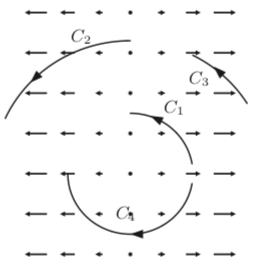
\includegraphics[width=2in]{img/C25p2-18.png}

\textbf{Extra}: For $C_1, C_2, C_4$, put the line integrals in order from least to greatest.


\vfill

\noindent\textbf{Circulation}.  A circulation integral is the line integral about a closed curve.  Let $C$ be a circle centered at the origin and oriented clockwise.  Identify the sign of the circulation around $C$ for each of the vector fields below.  \emph{pollQ}

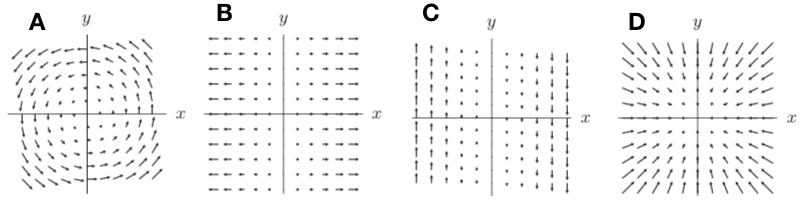
\includegraphics[width=\linewidth]{img/C25p4-18.png}
\vfill



\noindent\textbf{Line integrals}.  Pair the line integrals that are equal based on the diagrams below.

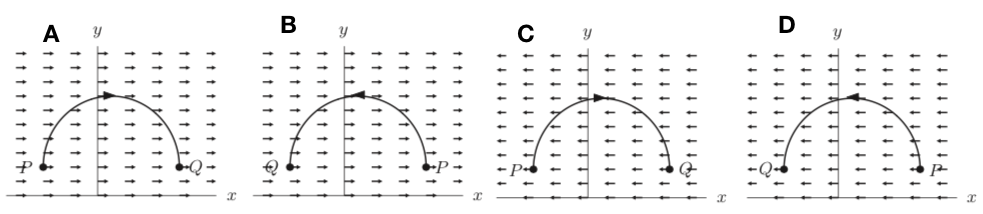
\includegraphics[width=\linewidth]{img/C25p5-18.png}

\vfill

%\eject
\noindent\textbf{Work done by a vector field}.  The work done by a force field is given by $\int_C \mb F\cdot d\mb r$.  Let $\mb F = y\mb i$ be a force field.  An object moves along a straight line joining $(1,1)$ to $(1,-1)$.  Find the sign of the work done by the force field. % \emph{pollQ}


\textbf{Extra:} Give paths for which the other cases would occur.  Give vector fields for which the other cases would occur.

\vfill

\eject

% \noindent\textbf{Gradient field}.  Let $\mb F = \mb \nabla f$ for some function $f$, so $\mb F$ is a gradient field.  Consider $\int_C \mb\nabla f\cdot d\mb r$.  Recall $\int_C \mb \nabla f \cdot d\mb r = \int_C \mb \nabla f\cdot \mb T\ ds$.  A Riemann sum approximation for the line integral is $\sum \mb\nabla f(\mb r_i)\cdot \mb T \Delta s_i$.  Which of the following statements hold?

% \begin{enumerate}
%     \item On a segment $\Delta s_i$ where $C$ crosses a level curve of $f$ in a direction where $f$ is increasing, there is a positive contribution to the Riemann sum.
%     \item On a segment $\Delta s_i$ where $f$ is positive there is a positive contribution to the Riemann sum.
%     \item On a segment $\Delta s_i$ where $C$ is tangent to a level curve of $f$ there is a positive contribution to the Riemann sum.
% \end{enumerate}

% \vfill

\noindent\textbf{Problem}.  Let $C$ be the line segment from the origin to $(1,1,1)$.  Let $\mb F = ay\mb i -ax\mb j + (b-1)\mb k$.  Give conditions on $a$ and $b$ so that the line integral $\int_C \mb F\cdot d\mb r$ is positive.
\vfill


\vspace{0.2cm}
\hrule
\vspace{0.2cm}







\end{document}